% ============================================================================
% DÉFINITION DU COURS 02 : MODÉLISATION DES MÉCANISMES
% Couverture, cours et exercices. Les packages sont chargés par le fichier 00.
% ============================================================================

% Illustration de réflexion issue du document Word.
\TLSetReflectionImage{images/image60.png}

\titlehead{Thomas Lusseau - SII en ATS}
\title[Modélisation des mécanismes]{Modélisation des mécanismes}
\author[TL]{Thomas Lusseau}
\date{\today}

\TLCourseCoverSetup
  {\repStyle/FondPoly.png}
  {images/image3.png}
  {Cycle 2 : Modéliser et déterminer les lois de\\ mouvement d'un mécanisme}
  {Modélisation des mécanismes}
  {Lycée Robert Doisneau - ATS}
  {Thomas Lusseau}

\TLCourseCoverContents{%
  \TLCourseContentsLine{2.1}{MISE EN SITUATION}{TL-course-section-1}
  \TLCourseContentsLine{2.2}{Introduction à la modélisation cinématique}{TL-course-section-2}
  \TLCourseContentsLine{2.3}{Les liaisons cinématiques}{TL-course-section-3}
  \TLCourseContentsLine{2.4}{Élaboration d'un modèle cinématique}{TL-course-section-4}
  \TLCourseContentsLine{2.5}{Paramétrage d'un schéma cinématique}{TL-course-section-5}
  \TLCourseContentsLine{2.6}{Liaison équivalente}{TL-course-section-6}
  \TLCourseContentsLine{2.7}{Sources}{TL-course-section-7}
  \TLCourseContentsLine{2.8}{Exercices du chapitre}{exercices-du-chapitre}
}

\TLCourseFooter
\TLCourseCover
\markboth{Modélisation des mécanismes}{Modélisation des mécanismes}

\AtBeginEnvironment{corrige}{\small}
\livrettrue
%\livretfalse
\collefalse

% Cours recomposé à partir du document Word d'origine.
% ============================================================================
% COURS 02 — MODÉLISATION DES MÉCANISMES
% Recomposition fidèle du document Word 2-ModelisationMecanismes2022.docx.
% Les schémas de liaisons normalisées utilisent Style/cinematique.sty.
% ============================================================================

\pagelayout{wide}
\setcounter{chapter}{2}
\setcounter{section}{0}

\definecolor{TLCycleBlue}{RGB}{78,139,199}
\definecolor{TLSectionBlue}{RGB}{35,146,166}
\definecolor{TLSubsectionOrange}{RGB}{203,118,0}
\definecolor{TLDefinitionPurple}{RGB}{115,55,155}
\definecolor{TLSoftOrange}{RGB}{252,238,224}
\definecolor{TLSoftBlue}{RGB}{235,244,250}
\definecolor{TLTableHeader}{RGB}{202,218,238}

\newcommand{\TLCheck}{\(\bigcirc\)}
\newcommand{\TLImage}[2][0.88\linewidth]{%
  \begin{center}
    \includegraphics[width=#1,height=.34\textheight,keepaspectratio]{#2}
  \end{center}
}
\newcommand{\TLImageSmall}[2][0.58\linewidth]{%
  \begin{center}
    \includegraphics[width=#1,height=.25\textheight,keepaspectratio]{#2}
  \end{center}
}
\newcommand{\TLSectionLabel}[1]{\label{TL-course-section-#1}}

\newtcolorbox{TLDefinition}[1][Définition]{
  enhanced,breakable,
  colback=TLDefinitionPurple!5,
  colframe=TLDefinitionPurple,
  boxrule=.9pt,arc=3mm,
  title={#1},
  colbacktitle=TLDefinitionPurple!8,
  coltitle=TLDefinitionPurple,
  fonttitle=\bfseries,
  attach boxed title to top center={yshift=-2mm},
  boxed title style={arc=2mm,boxrule=.9pt},
  left=4mm,right=4mm,top=4mm,bottom=3mm
}
\newtcolorbox{TLRemark}[1][Remarque]{
  enhanced,breakable,
  colback=TLSoftBlue,
  colframe=TLCoverBlue,
  boxrule=.7pt,arc=2mm,
  title={#1},fonttitle=\bfseries,
  colbacktitle=TLCoverBlue,coltitle=white,
  left=4mm,right=4mm,top=3mm,bottom=3mm
}
\newtcolorbox{TLQuoteBox}{
  enhanced,breakable,
  colback=TLSoftOrange,
  colframe=TLSubsectionOrange!65!black,
  boxrule=.6pt,arc=2mm,
  left=8mm,right=8mm,top=5mm,bottom=5mm,
  fontupper=\large\centering
}

% Symboles normalisés issus de cinematique.sty.
\newcommand{\TLSymPivot}{%
  \begin{tikzpicture}[baseline=-.5ex,scale=.65]\scPivotx{L}{(0,0)}\end{tikzpicture}}
\newcommand{\TLSymPivotGlissant}{%
  \begin{tikzpicture}[baseline=-.5ex,scale=.65]\scPivotGlissantx{L}{(0,0)}\end{tikzpicture}}
\newcommand{\TLSymGlissiere}{%
  \begin{tikzpicture}[baseline=-.5ex,scale=.65]\scGlissierex{L}{(0,0)}\end{tikzpicture}}
\newcommand{\TLSymHelicoidale}{%
  \begin{tikzpicture}[baseline=-.5ex,scale=.65]\scHelicoidalex{L}{(0,0)}\end{tikzpicture}}
\newcommand{\TLSymAppuiPlan}{%
  \begin{tikzpicture}[baseline=-.5ex,scale=.70]\scAppuiPlan{L}{(0,0)}\end{tikzpicture}}
\newcommand{\TLSymSpherePlan}{%
  \begin{tikzpicture}[baseline=-.5ex,scale=.70]\scSpherePlan{L}{(0,0)}\end{tikzpicture}}
\newcommand{\TLSymCylindrePlan}{%
  \begin{tikzpicture}[baseline=-.5ex,scale=.70]\scCylindrePlanx{L}{(0,0)}\end{tikzpicture}}
\newcommand{\TLSymSphereCylindre}{%
  \begin{tikzpicture}[baseline=-.5ex,scale=.70]\scSphereCylindrex{L}{(0,0)}\end{tikzpicture}}
\newcommand{\TLSymSpherique}{%
  \begin{tikzpicture}[baseline=-.5ex,scale=.70]\scSpherique{L}{(0,0)}\end{tikzpicture}}
\newcommand{\TLSymSpheriqueDoigt}{%
  \begin{tikzpicture}[baseline=-.5ex,scale=.70]\scSpheriqueDoigt{L}{(0,0)}\end{tikzpicture}}

\newcommand{\TLTorseur}[7]{%
  \(\left\{\mathcal V\right\}
  =\left\{\begin{array}{cc}
  #1 & #4\\
  #2 & #5\\
  #3 & #6
  \end{array}\right\}_{#7}\)
}

% Bandeau de cycle, fidèle au document Word, sur les pages de contenu.
\newcommand{\TLModelisationHeader}{%
  \ifnum\value{page}>1\relax
  \begin{tikzpicture}[remember picture,overlay]
    \fill[TLCycleBlue]
      ([xshift=82mm,yshift=-10mm]current page.north west)
      -- ([xshift=94mm,yshift=-3mm]current page.north west)
      -- ([yshift=-3mm]current page.north east)
      -- ([yshift=-17mm]current page.north east)
      -- ([xshift=82mm,yshift=-17mm]current page.north west) -- cycle;
    \node[anchor=east,text=white,font=\sffamily\bfseries\small,xshift=-9mm,yshift=-10mm]
      at (current page.north east) {Cycle 2 : Modélisation des mécanismes};
  \end{tikzpicture}%
  \fi
}
\AddToShipoutPictureFG{\TLModelisationHeader}

\section*{Objectifs du cours}
\addcontentsline{toc}{section}{Objectifs du cours}

\begin{tcolorbox}[
  enhanced,breakable,
  colback=white,colframe=TLCoverBlue,
  boxrule=.8pt,arc=2mm,
  title={Modéliser et analyser le comportement cinématique d'un mécanisme},
  colbacktitle=TLCoverBlue,coltitle=white,fonttitle=\bfseries
]
L'objectif est de savoir construire et exploiter un \textbf{schéma cinématique}
et/ou un \textbf{graphe de liaisons}.
\end{tcolorbox}

\begin{minipage}[t]{.48\linewidth}
\textbf{\large Savoirs — Je connais :}
\begin{itemize}
  \item les noms des dix liaisons usuelles ; \hfill\TLCheck
  \item leurs symboles de représentation 2D et 3D ; \hfill\TLCheck
  \item la forme générale de leurs torseurs cinématiques ; \hfill\TLCheck
  \item les symboles des transmetteurs usuels ; \hfill\TLCheck
  \item la modélisation des guidages par roulements ; \hfill\TLCheck
  \item la démarche d'élaboration d'un schéma cinématique. \hfill\TLCheck
\end{itemize}
\end{minipage}\hfill
\begin{minipage}[t]{.48\linewidth}
\textbf{\large Savoir-faire — Je sais :}
\begin{itemize}
  \item identifier et caractériser une liaison usuelle ; \hfill\TLCheck
  \item repérer les classes d'équivalence cinématique ; \hfill\TLCheck
  \item identifier la géométrie d'un contact ; \hfill\TLCheck
  \item modéliser les mouvements relatifs entre deux CEC ; \hfill\TLCheck
  \item réaliser un graphe des liaisons ; \hfill\TLCheck
  \item élaborer un schéma cinématique ; \hfill\TLCheck
  \item déterminer une liaison équivalente. \hfill\TLCheck
\end{itemize}
\end{minipage}

\section{MISE EN SITUATION}\TLSectionLabel{1}

\subsection{Cas n\textsuperscript{o}1 : lenteur d'un robot de chirurgie}

Même si elle n'est pas encore aussi répandue en France qu'aux États-Unis,
la chirurgie robotique se développe progressivement. Son usage nécessite
la maîtrise de la machine et une familiarisation avec sa manipulation,
mais également la prise en compte de contraintes telles que la durée de
l'intervention. Un arrêt de la cour administrative d'appel de Lyon du
29 septembre 2016 rappelle que l'allongement de la durée d'une opération,
lié à l'installation du robot et à un maniement hésitant, peut être en lien
direct avec les dommages subis.

\TLImage[.72\linewidth]{images/image5.jpeg}

Pour de nombreux systèmes, en particulier en robotique industrielle ou
grand public, un enjeu majeur consiste à respecter la \textbf{cinématique}
imposée par le cahier des charges : mouvements suivant des directions
déterminées, amplitudes et vitesses maîtrisées.

\TLImage[.76\linewidth]{images/image6.png}

On cherche donc à établir des relations entre les \textbf{ordres} envoyés
aux pré-actionneurs de la chaîne de puissance et la
\textbf{cinématique imposée aux effecteurs}.

\subsection{Cas n\textsuperscript{o}2 : prothèse transtibiale}

La prothèse transtibiale doit permettre à la personne de réaliser des
mouvements comparables à ceux d'un pied réel, en termes d'amplitude,
de vitesse et d'accélération.

\begin{center}
\begin{minipage}{.43\linewidth}\centering
  
\includegraphics[width=.72\linewidth,height=.24\textheight,keepaspectratio]{images/image7.jpeg}\\
  \emph{Prothèse transtibiale}
\end{minipage}\hfill
\begin{minipage}{.53\linewidth}
\begin{TLQuoteBox}
Pour maîtriser les positions et les vitesses, il faut pouvoir
\textbf{modéliser les différents mouvements du mécanisme}.
\end{TLQuoteBox}
\end{minipage}
\end{center}

\section{INTRODUCTION À LA MODÉLISATION CINÉMATIQUE}\TLSectionLabel{2}

\subsection{Définitions et hypothèses}

\begin{TLDefinition}
\textbf{Mécanisme :} ensemble des solides de la chaîne de puissance situés
entre l'actionneur et l'effecteur, assurant le transfert de puissance mécanique.
\end{TLDefinition}

\begin{TLDefinition}
\textbf{Solide ou classe d'équivalence cinématique (CEC) :} pièce ou ensemble
de pièces assemblées entre elles et ne présentant aucun mouvement relatif.
\end{TLDefinition}

Lors de l'utilisation d'un mécanisme, les solides se déforment sous l'action
des efforts. Dans ce cours, ces déformations sont supposées suffisamment
faibles pour être négligées : les solides sont considérés
\textbf{indéformables}.

\begin{TLDefinition}
Un solide indéformable \(S\) vérifie :
\[
\forall t,\ \forall A,B\in S,\qquad AB=\text{constante}.
\]
\end{TLDefinition}

\begin{TLRemark}
Cette hypothèse ne convient pas aux pièces dont la fonction est précisément
de se déformer : ressorts, barres de torsion, rondelles élastiques, etc.
\end{TLRemark}

\subsection{Modèle cinématique}

L'étude du comportement cinématique d'un mécanisme s'appuie sur un modèle,
généralement constitué d'un \textbf{schéma cinématique} et/ou d'un
\textbf{graphe des liaisons}.

\TLImage[.78\linewidth]{images/image12.png}

Ces représentations simplifiées sont utilisées aussi bien pour analyser un
système existant que pour concevoir un nouveau système. Elles constituent
des outils efficaces de communication scientifique.

\subsection{Schéma cinématique d'un mécanisme}

Un schéma cinématique propose une représentation géométrique du modèle.
Il précise les mouvements possibles entre les solides, les liaisons et les
positions relatives de ces liaisons dans l'espace.

\begin{itemize}
  \item les liaisons sont représentées par des symboles normalisés ;
  \item les solides sont représentés par des traits reliant ces symboles.
\end{itemize}

\begin{center}
\begin{minipage}[t]{.46\linewidth}\centering
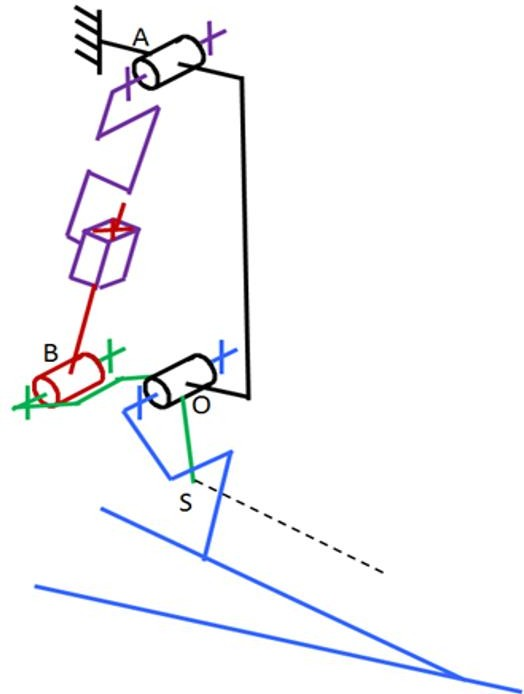
\includegraphics[width=\linewidth,height=.28\textheight,keepaspectratio]{images/image14.jpeg}\\
\emph{Schéma cinématique 3D}
\end{minipage}\hfill
\begin{minipage}[t]{.46\linewidth}\centering
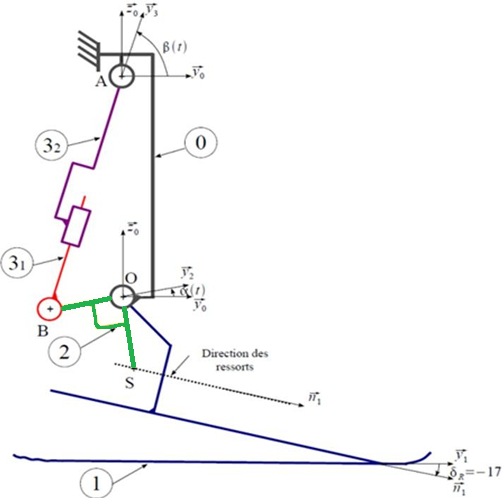
\includegraphics[width=\linewidth,height=.28\textheight,keepaspectratio]{images/image13.png}\\
\emph{Schéma cinématique 2D}
\end{minipage}
\end{center}

Le schéma peut être plan ou spatial. Il comporte également les points,
vecteurs et droites nécessaires au paramétrage.

\subsection{Graphe de liaisons d'un mécanisme}

Un graphe des liaisons représente les CEC par des nœuds et les liaisons par
des arêtes portant leurs caractéristiques géométriques.

\begin{TLQuoteBox}
Une liaison entre deux solides possède toujours exactement deux couleurs.
\end{TLQuoteBox}

\begin{center}
\begin{minipage}[t]{.56\linewidth}\centering
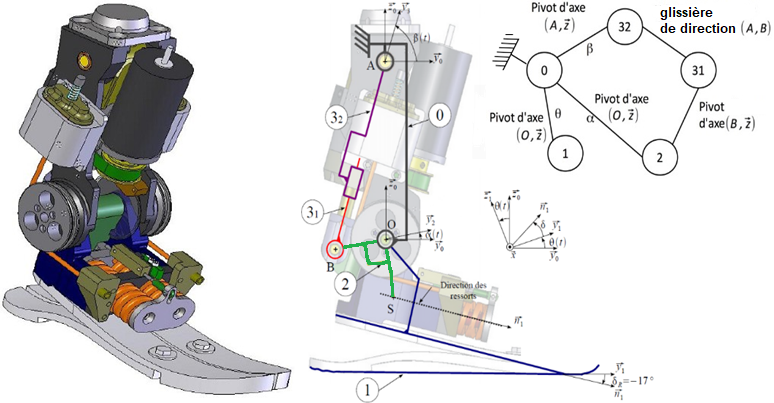
\includegraphics[width=\linewidth,height=.27\textheight,keepaspectratio]{images/image12.png}
\end{minipage}\hfill
\begin{minipage}[t]{.38\linewidth}
\begin{itemize}
  \item les solides sont les \textbf{nœuds} ;
  \item les liaisons sont les \textbf{arêtes} ;
  \item le bâti est le solide de référence.
\end{itemize}
\end{minipage}
\end{center}

Le graphe est plus simple à tracer car il ne représente pas la géométrie.
Il contient néanmoins la même information cinématique que le schéma associé.

\subsubsection*{Chaînes de solides ouvertes, fermées et complexes}

\begin{tabularx}{\linewidth}{|>{\centering\arraybackslash}X|>{\centering\arraybackslash}X|>{\centering\arraybackslash}X|}
\hline
\rowcolor{TLTableHeader}
\textbf{Chaîne ouverte} & \textbf{Chaîne fermée} & \textbf{Chaîne complexe}\\ \hline
Les solides extrêmes sont différents. &
Le solide initial est aussi le solide final. &
Plusieurs chaînes ouvertes ou fermées sont associées.\\

\includegraphics[width=.32\linewidth]{images/image15.png} &

\includegraphics[width=.32\linewidth]{images/image15.png} &

\includegraphics[width=.32\linewidth]{images/image15.png}\\
Exemple : robot & Exemple : antenne radar & Exemple : simulateur de vol\\ \hline
\end{tabularx}

% ============================================================================
% SYMBOLES DE LIAISONS — BIBLIOTHÈQUE CINÉMATIQUE
% Les commandes de cinematique.sty attendent les coordonnées sans parenthèses
% dans leur troisième argument : {0,0} et non {(0,0)}.
% ============================================================================

\renewcommand{\TLSymPivot}{%
  \begin{tikzpicture}[baseline=-.5ex,scale=.65]
    \scPivotx{L}{0,0}
  \end{tikzpicture}%
}

\renewcommand{\TLSymPivotGlissant}{%
  \begin{tikzpicture}[baseline=-.5ex,scale=.65]
    \scPivotGlissantx{L}{0,0}
  \end{tikzpicture}%
}

\renewcommand{\TLSymGlissiere}{%
  \begin{tikzpicture}[baseline=-.5ex,scale=.65]
    \scGlissierex{L}{0,0}
  \end{tikzpicture}%
}

\renewcommand{\TLSymHelicoidale}{%
  \begin{tikzpicture}[baseline=-.5ex,scale=.65]
    \scHelicoidalex{L}{0,0}
  \end{tikzpicture}%
}

\renewcommand{\TLSymAppuiPlan}{%
  \begin{tikzpicture}[baseline=-.5ex,scale=.70]
    \scAppuiPlan{L}{0,0}
  \end{tikzpicture}%
}

\renewcommand{\TLSymSpherePlan}{%
  \begin{tikzpicture}[baseline=-.5ex,scale=.70]
    \scSpherePlan{L}{0,0}
  \end{tikzpicture}%
}

\renewcommand{\TLSymCylindrePlan}{%
  \begin{tikzpicture}[baseline=-.5ex,scale=.70]
    \scCylindrePlanx{L}{0,0}
  \end{tikzpicture}%
}

\renewcommand{\TLSymSphereCylindre}{%
  \begin{tikzpicture}[baseline=-.5ex,scale=.70]
    \scSphereCylindrex{L}{0,0}
  \end{tikzpicture}%
}

\renewcommand{\TLSymSpherique}{%
  \begin{tikzpicture}[baseline=-.5ex,scale=.70]
    \scSpherique{L}{0,0}
  \end{tikzpicture}%
}

\renewcommand{\TLSymSpheriqueDoigt}{%
  \begin{tikzpicture}[baseline=-.5ex,scale=.70]
    \scSpheriqueDoigt{L}{0,0}
  \end{tikzpicture}%
}

\section{LES LIAISONS CINÉMATIQUES}\TLSectionLabel{3}

\subsection{Introduction}

Une liaison est un \textbf{modèle du comportement cinématique} d'un solide
par rapport à un autre. Elle définit les mouvements relatifs possibles,
indépendamment de la réalisation technologique : contact direct, coussinet,
roulement, etc.

\begin{center}
\begin{minipage}{.56\linewidth}
Différentes réalités technologiques peuvent donc conduire au même
comportement cinématique et à la même liaison.
\end{minipage}\hfill
\begin{minipage}{.40\linewidth}\centering
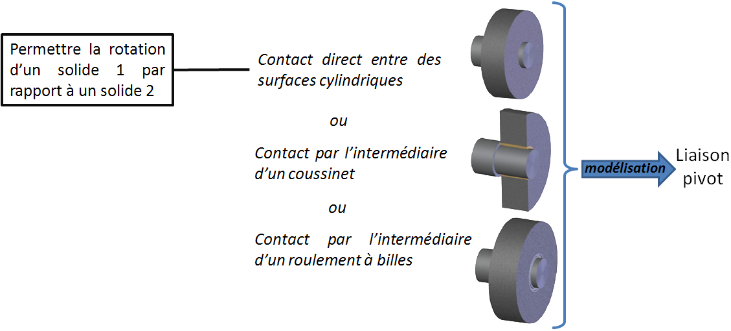
\includegraphics[width=\linewidth,height=.20\textheight,keepaspectratio]{images/image19.png}
\end{minipage}
\end{center}

\subsection{Degrés de liberté}

\begin{TLDefinition}
Un \textbf{degré de liberté} est un mouvement relatif élémentaire indépendant
autorisé par une liaison. Les six mouvements élémentaires sont les trois
translations \(T_x,T_y,T_z\) et les trois rotations \(R_x,R_y,R_z\).
\end{TLDefinition}

\begin{center}
\begin{tabular}{|c|p{.60\linewidth}|}
\hline
\rowcolor{TLTableHeader}\textbf{Mouvement} & \textbf{Signification}\\ \hline
\(T_x,T_y,T_z\) & translations rectilignes suivant \(\vec x,\vec y,\vec z\)\\ \hline
\(R_x,R_y,R_z\) & rotations autour des axes \((O,\vec x),(O,\vec y),(O,\vec z)\)\\ \hline
\end{tabular}\qquad

\includegraphics[width=.22\linewidth,height=.17\textheight,keepaspectratio]{images/image26.png}
\end{center}

Le nombre de degrés de liberté est le nombre de paramètres indépendants
nécessaires pour caractériser le mouvement relatif entre les deux solides.

\subsection{Description d'une liaison}

Pour chacune des liaisons, on associe les informations suivantes.

\begin{tabularx}{\linewidth}{|>{\bfseries}p{.28\linewidth}|X|}
\hline
\rowcolor{TLTableHeader}Élément & Remarques\\ \hline
Nom & Deux désignations peuvent parfois correspondre à une même liaison.\\ \hline
Description géométrique & Axe pour un cylindre, normale pour un plan, centre pour une sphère.\\ \hline
Symboles 2D et 3D & Ils expriment uniquement les mouvements possibles et non la réalisation matérielle.\\ \hline
Mobilités / degrés de liberté & Tableau des rotations et translations autorisées.\\ \hline
Paramétrage & Position linéaire ou angulaire relative ; les rotations sont représentées sur une figure de changement de base.\\ \hline
Torseur cinématique & Forme générale exprimée en un point caractéristique de la liaison.\\ \hline
\end{tabularx}

\subsection{Liaisons simples}

Les liaisons simples proviennent de l'association de surfaces élémentaires :
plan, cylindre et sphère.

\begin{center}
\begin{tabularx}{.96\linewidth}{|c|>{\centering\arraybackslash}X|>{\centering\arraybackslash}X|>{\centering\arraybackslash}X|}
\hline
 & \textbf{Plan} & \textbf{Sphère} & \textbf{Cylindre}\\ \hline
\textbf{Plan}
& 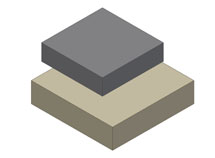
\includegraphics[width=.55\linewidth]{images/image37.jpeg}\\Appui-plan\\contact surfacique
& 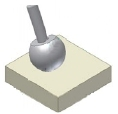
\includegraphics[width=.55\linewidth]{images/image38.jpeg}\\Sphère-plan\\contact ponctuel
& 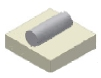
\includegraphics[width=.55\linewidth]{images/image39.jpeg}\\Cylindre-plan\\contact linéique\\ \hline
\textbf{Sphère}
& 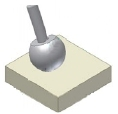
\includegraphics[width=.55\linewidth]{images/image38.jpeg}\\Sphère-plan
& 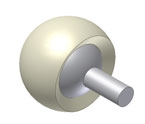
\includegraphics[width=.55\linewidth]{images/image40.jpeg}\\Sphérique
& 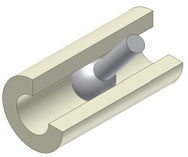
\includegraphics[width=.55\linewidth]{images/image41.jpeg}\\Sphère-cylindre\\ \hline
\textbf{Cylindre}
& 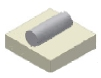
\includegraphics[width=.55\linewidth]{images/image39.jpeg}\\Cylindre-plan
& 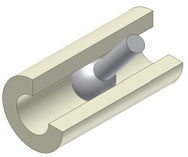
\includegraphics[width=.55\linewidth]{images/image41.jpeg}\\Sphère-cylindre
& 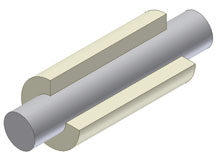
\includegraphics[width=.55\linewidth]{images/image42.jpeg}\\Pivot glissant\\ \hline
\end{tabularx}
\end{center}

\begin{longtable}{|p{.22\linewidth}|>{\centering\arraybackslash}p{.15\linewidth}|p{.15\linewidth}|p{.34\linewidth}|}
\hline
\rowcolor{TLTableHeader}
\textbf{Liaison} & \textbf{Symbole} & \textbf{Mobilité} & \textbf{Torseur cinématique}\\ \hline
\endfirsthead
\hline\rowcolor{TLTableHeader}
\textbf{Liaison} & \textbf{Symbole} & \textbf{Mobilité} & \textbf{Torseur cinématique}\\ \hline
\endhead
Appui-plan de normale \(\vec z\) &
\TLSymAppuiPlan &
\(R_z,T_x,T_y\) — 3 ddl &
\TLTorseur{\omega_x}{\omega_y}{\omega_z}{v_x}{v_y}{0}{P,\mathcal B}\\ \hline
Sphère-plan de normale \(\vec z\) &
\TLSymSpherePlan &
\(R_x,R_y,R_z,T_x,T_y\) — 5 ddl &
\TLTorseur{\omega_x}{\omega_y}{\omega_z}{v_x}{v_y}{0}{P,\mathcal B}\\ \hline
Sphère-cylindre d'axe \(\vec z\) &
\TLSymSphereCylindre &
4 ddl &
\TLTorseur{\omega_x}{\omega_y}{\omega_z}{0}{0}{v_z}{O,\mathcal B}\\ \hline
Cylindre-plan d'axe \(\vec x\), normale \(\vec z\) &
\TLSymCylindrePlan &
4 ddl &
\TLTorseur{\omega_x}{0}{\omega_z}{v_x}{v_y}{0}{P,\mathcal B}\\ \hline
Sphérique de centre \(O\) &
\TLSymSpherique &
\(R_x,R_y,R_z\) — 3 ddl &
\TLTorseur{\omega_x}{\omega_y}{\omega_z}{0}{0}{0}{O,\mathcal B}\\ \hline
Pivot glissant d'axe \(\vec z\) &
\TLSymPivotGlissant &
\(R_z,T_z\) — 2 ddl &
\TLTorseur{0}{0}{\omega_z}{0}{0}{v_z}{P,\mathcal B}\\ \hline
\end{longtable}

\TLReflectionBox{Compléter le tableau de mobilités et les symboles manquants, puis vérifier la cohérence avec les formes générales des torseurs cinématiques.}

\subsection{Liaisons composées}

Les liaisons composées résultent de plusieurs contacts élémentaires en série
ou en parallèle : glissière, pivot, hélicoïdale et sphérique à doigt.

\begin{center}
\begin{tabular}{cccc}
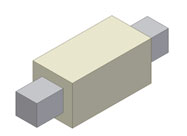
\includegraphics[width=.18\linewidth]{images/image61.jpeg} &

\includegraphics[width=.18\linewidth]{images/image62.jpeg} &
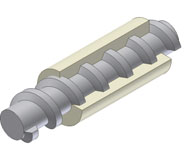
\includegraphics[width=.18\linewidth]{images/image63.jpeg} &
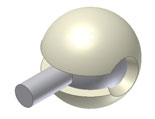
\includegraphics[width=.18\linewidth]{images/image64.jpeg}\\
\textbf{Glissière} & \textbf{Pivot} & \textbf{Hélicoïdale} & \textbf{Sphérique à doigt}
\end{tabular}
\end{center}

\begin{longtable}{|p{.22\linewidth}|>{\centering\arraybackslash}p{.15\linewidth}|p{.15\linewidth}|p{.34\linewidth}|}
\hline
\rowcolor{TLTableHeader}
\textbf{Liaison} & \textbf{Symbole} & \textbf{Mobilité} & \textbf{Torseur cinématique}\\ \hline
\endfirsthead
\hline\rowcolor{TLTableHeader}
\textbf{Liaison} & \textbf{Symbole} & \textbf{Mobilité} & \textbf{Torseur cinématique}\\ \hline
\endhead
Glissière de direction \(\vec z\) &
\TLSymGlissiere &
\(T_z\) — 1 ddl &
\TLTorseur{0}{0}{0}{0}{0}{v_z}{P,\mathcal B}\\ \hline
Pivot d'axe \((O,\vec z)\) &
\TLSymPivot &
\(R_z\) — 1 ddl &
\TLTorseur{0}{0}{\omega_z}{0}{0}{0}{P,\mathcal B}\\ \hline
Hélicoïdale d'axe \((O,\vec z)\) &
\TLSymHelicoidale &
\(R_z,T_z\) liés — 1 ddl &
\(v_z=p\,\omega_z\), avec \(p\) le pas réduit\\ \hline
Sphérique à doigt de centre \(O\), rotation \(\vec z\) interdite &
\TLSymSpheriqueDoigt &
2 ddl &
\TLTorseur{\omega_x}{\omega_y}{0}{0}{0}{0}{O,\mathcal B}\\ \hline
\end{longtable}

\begin{TLQuoteBox}
Pour un appui-plan, la seule rotation autorisée est celle autour de la
normale. Pour une liaison cylindre-plan, la seule translation impossible
est celle suivant la normale.
\end{TLQuoteBox}

% -----------------------------------------------------------------------------

\section{ÉLABORATION D'UN MODÈLE CINÉMATIQUE}\TLSectionLabel{4}

\subsection{Démarche}

\subsubsection*{Étape 1 — Identifier les classes d'équivalence cinématique}

Repérer les pièces ne présentant aucun mouvement relatif, les colorier,
nommer les CEC \(S_0,S_1,\ldots\) et lister les pièces qui les constituent.

\begin{center}
\begin{minipage}{.57\linewidth}
\begin{itemize}
  \item exclure les pièces déformables : ressorts, joints, rondelles élastiques ;
  \item exclure les éléments roulants : billes, rouleaux, aiguilles ;
  \item choisir un bâti unique, considéré fixe dans le référentiel d'étude.
\end{itemize}
\end{minipage}\hfill
\begin{minipage}{.38\linewidth}\centering
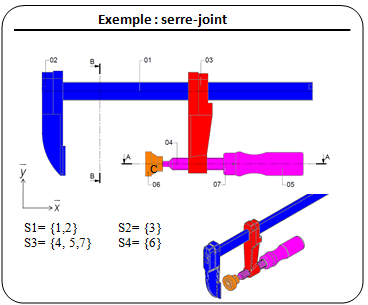
\includegraphics[width=\linewidth,height=.22\textheight,keepaspectratio]{images/image80.png}
\end{minipage}
\end{center}

\subsubsection*{Étape 2 — Réaliser le graphe des liaisons}

\begin{itemize}
  \item représenter chaque CEC par une bulle ;
  \item identifier le bâti ;
  \item identifier les contacts et les mouvements relatifs ;
  \item relier les bulles et préciser le nom et les éléments géométriques des liaisons.
\end{itemize}

\TLImageSmall[.55\linewidth]{images/image84.png}

Deux questions guident l'identification : quelle est la nature des surfaces
en contact ? Quels sont les mouvements relatifs possibles ?

\subsubsection*{Étape 3 — Élaborer le schéma cinématique}

Positionner les centres et les axes, placer les symboles normalisés avec le
code couleur, relier les éléments de même couleur et vérifier la cohérence
avec les mouvements réels.

\TLImageSmall[.60\linewidth]{images/image3.png}

\begin{TLRemark}
Lorsque le graphe a été simplifié grâce aux liaisons équivalentes, le schéma
obtenu est un \textbf{schéma cinématique minimal}.
\end{TLRemark}

\subsubsection*{Application : micromoteur}

Le micromoteur comporte quatre CEC : le carter \(0\), le vilebrequin \(1\),
la bielle \(2\) et le piston \(3\).

\begin{center}
\begin{minipage}[t]{.47\linewidth}\centering
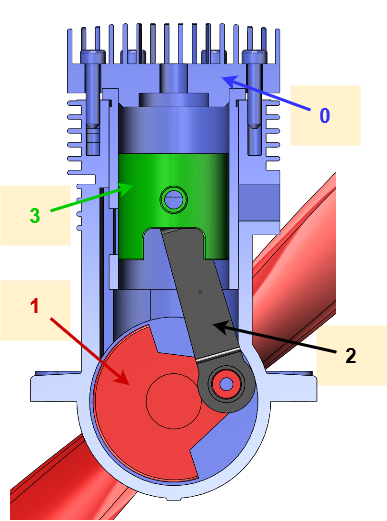
\includegraphics[width=.92\linewidth,height=.28\textheight,keepaspectratio]{images/image86.png}\\
\emph{Identification des CEC et points caractéristiques}
\end{minipage}\hfill
\begin{minipage}[t]{.47\linewidth}\centering
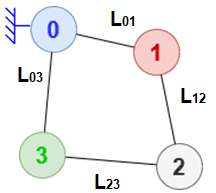
\includegraphics[width=.88\linewidth,height=.28\textheight,keepaspectratio]{images/image87.png}\\
\emph{Graphe des liaisons}
\end{minipage}
\end{center}

Les liaisons sont :
\[
L_{01}\text{ pivot en }A,\quad
L_{12}\text{ pivot en }B,\quad
L_{23}\text{ pivot glissant en }C,\quad
L_{30}\text{ pivot glissant en }A.
\]

\TLImageSmall[.55\linewidth]{images/image93.png}

\subsection{Modélisation des guidages}

Grâce à des éléments glissants ou roulants, on obtient des mouvements
relatifs plus performants du point de vue énergétique.

\begin{tabularx}{\linewidth}{|>{\centering\arraybackslash}p{.32\linewidth}|X|}
\hline
\rowcolor{gray!25}\textbf{Coussinets} & \textbf{Modélisation}\\ \hline

\includegraphics[width=.74\linewidth]{images/image95.png}\quad
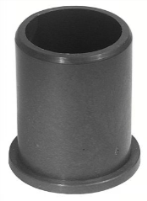
\includegraphics[width=.74\linewidth]{images/image96.png}
& Liaison pivot ou pivot glissant.\\ \hline
\end{tabularx}

\subsubsection*{Roulements}

Le choix entre pivot et sphérique dépend notamment de l'angle maximal de
rotulage. Le jeu interne autorise de faibles rotations autour des axes
secondaires.

\begin{tabularx}{\linewidth}{|>{\centering\arraybackslash}X|>{\centering\arraybackslash}X|}
\hline
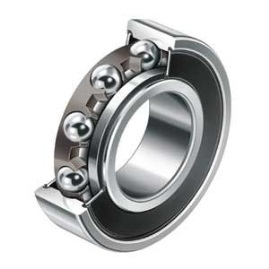
\includegraphics[width=.43\linewidth]{images/image99.jpeg}\quad
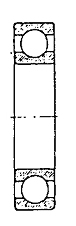
\includegraphics[width=.18\linewidth]{images/image100.jpeg}
&
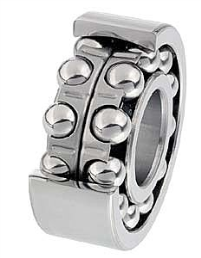
\includegraphics[width=.43\linewidth]{images/image101.png}\quad
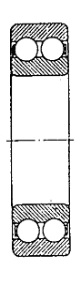
\includegraphics[width=.18\linewidth]{images/image102.jpeg}\\
Une rangée de billes : en général rotulage \(>5'\), modèle sphérique.
&
Deux rangées de billes : en général rotulage \(<5'\), modèle pivot.\\ \hline
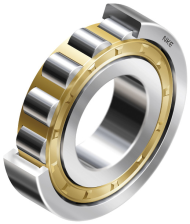
\includegraphics[width=.43\linewidth]{images/image103.png}\quad

\includegraphics[width=.30\linewidth]{images/image104.png}
&

\includegraphics[width=.43\linewidth]{images/image106.jpeg}\quad

\includegraphics[width=.18\linewidth]{images/image107.jpeg}\\
Aiguilles ou rouleaux : rotulage \(<5'\), modèle pivot.
&
Roulement à rotule : rotulage de \(2^\circ\) à \(4^\circ\), modèle sphérique.\\ \hline
\end{tabularx}

\begin{tabularx}{\linewidth}{|>{\bfseries}p{.30\linewidth}|X|}
\hline
Pivot & rotulage \(<5'\) et deux bagues arrêtées en translation.\\ \hline
Pivot glissant & rotulage \(<5'\) et une bague libre en translation.\\ \hline
Sphérique & rotulage \(>5'\) et deux bagues arrêtées en translation.\\ \hline
Sphère-cylindre & rotulage \(>5'\) et une bague libre en translation.\\ \hline
\end{tabularx}

\subsubsection*{Autres guidages}

\begin{tabularx}{\linewidth}{|>{\centering\arraybackslash}p{.34\linewidth}|X|}
\hline

\includegraphics[width=.72\linewidth]{images/image108.png}
& \textbf{Douille à billes :} pivot glissant.\\ \hline
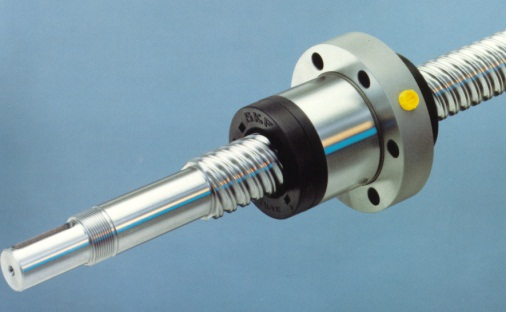
\includegraphics[width=.72\linewidth]{images/image110.jpeg}
& \textbf{Vis à billes :} hélicoïdale.\\ \hline
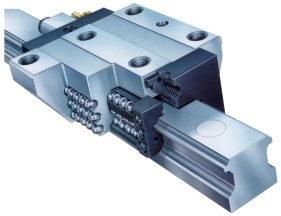
\includegraphics[width=.72\linewidth]{images/image111.jpeg}
& \textbf{Guidage à billes :} glissière.\\ \hline

\includegraphics[width=.36\linewidth]{images/image112.png}\quad
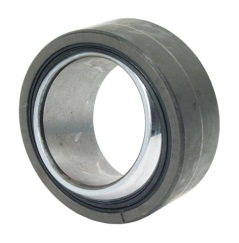
\includegraphics[width=.36\linewidth]{images/image113.jpeg}
& \textbf{Rotule lisse :} sphérique.\\ \hline
\end{tabularx}

\subsection{Modélisation des transmetteurs usuels}

\begin{tabularx}{\linewidth}{|>{\centering\arraybackslash}p{.32\linewidth}|>{\centering\arraybackslash}X|}
\hline
\rowcolor{gray!20}\textbf{Réalisation technologique} & \textbf{Schéma cinématique}\\ \hline
\textbf{Roue et vis sans fin}\\
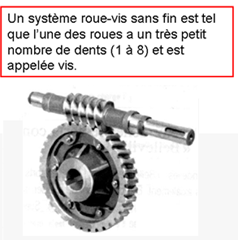
\includegraphics[width=.72\linewidth]{images/image115.png}
& 
\includegraphics[width=.70\linewidth]{images/image114.png}\\ \hline
\textbf{Poulie-courroie}\\
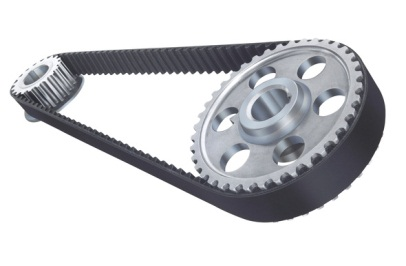
\includegraphics[width=.72\linewidth]{images/image117.jpeg}
& 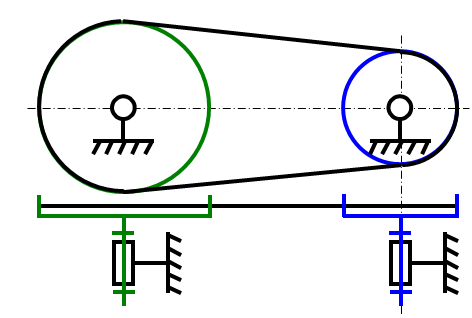
\includegraphics[width=.70\linewidth]{images/image116.png}\\ \hline
\textbf{Engrenages}\\

\includegraphics[width=.72\linewidth]{images/image119.png}
& 
\includegraphics[width=.70\linewidth]{images/image118.png}\\ \hline
\end{tabularx}

% -----------------------------------------------------------------------------
\section{PARAMÉTRAGE D'UN SCHÉMA CINÉMATIQUE}\TLSectionLabel{5}

Afin de simuler le comportement du mécanisme, on associe une base orthonormée
directe à chaque CEC. Le solide \(i\) reçoit le repère
\(\mathcal R_i=(O_i,\vec x_i,\vec y_i,\vec z_i)\).

\begin{center}
\begin{minipage}[t]{.48\linewidth}\centering

\includegraphics[width=.92\linewidth,height=.28\textheight,keepaspectratio]{images/image120.png}\\
\emph{Antenne parabolique}
\end{minipage}\hfill
\begin{minipage}[t]{.48\linewidth}\centering

\includegraphics[width=.92\linewidth,height=.28\textheight,keepaspectratio]{images/image121.png}\\
\emph{Échelle EPAS}
\end{minipage}
\end{center}

\subsection{Base orthonormée}

Une base associée à un solide est :
\begin{itemize}
  \item \textbf{orthonormée} : vecteurs orthogonaux deux à deux et unitaires ;
  \item \textbf{directe} : orientation donnée par la règle de la main droite.
\end{itemize}

\TLImageSmall[.34\linewidth]{images/image124.jpeg}

Les bases se déplacent avec les CEC. On utilise des paramètres de mouvement :
un angle pour une liaison pivot et une distance pour une glissière.

\subsection{Figures de changement de base}

Pour construire une figure de changement de base :
\begin{enumerate}
  \item dessiner un petit angle, de l'ordre de \(20^\circ\) ;
  \item placer face à soi le vecteur commun autour duquel la base tourne ;
  \item compléter les deux bases de manière directe ;
  \item reporter les égalités entre vecteurs unitaires.
\end{enumerate}

\TLImageSmall[.42\linewidth]{images/image125.jpeg}

Il faut une figure par liaison pivot. Lorsque plusieurs pivots ont des axes
parallèles, les figures peuvent être superposées.

\TLReflectionBox{Réaliser les figures de changement de base de l'antenne parabolique et de l'échelle EPAS, puis celles du robot de soudage.}

\begin{center}
\begin{minipage}[t]{.43\linewidth}\centering
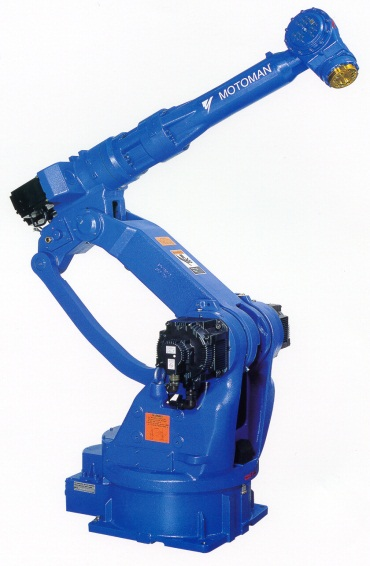
\includegraphics[width=.84\linewidth,height=.26\textheight,keepaspectratio]{images/image140.jpeg}\\
\emph{Robot de soudage}
\end{minipage}\hfill
\begin{minipage}[t]{.53\linewidth}\centering
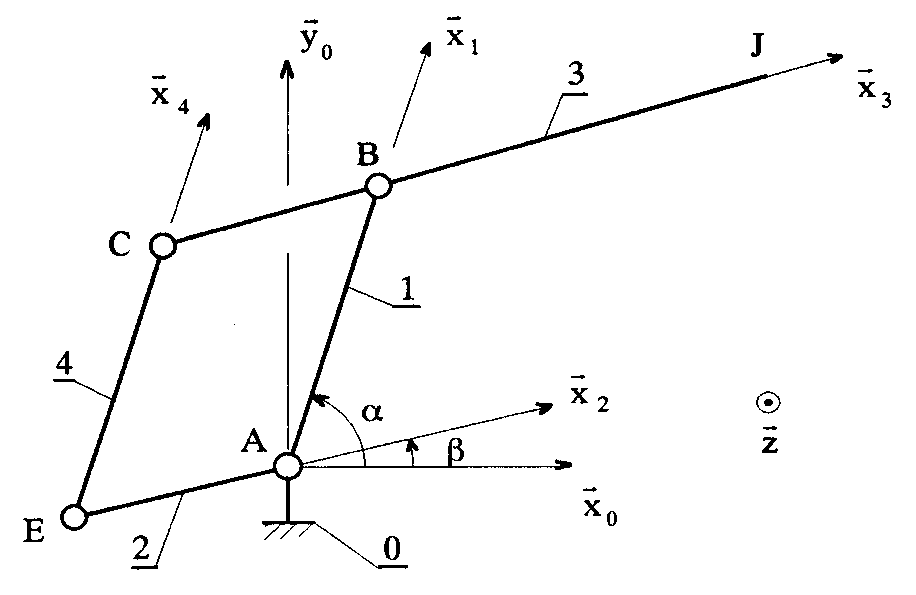
\includegraphics[width=\linewidth,height=.26\textheight,keepaspectratio]{images/image139.png}\\
\emph{Paramétrage du mécanisme}
\end{minipage}
\end{center}

% -----------------------------------------------------------------------------
\section{LIAISON ÉQUIVALENTE}\TLSectionLabel{6}

Une liaison équivalente à plusieurs liaisons entre deux CEC traduit le même
mouvement relatif et permet de transmettre les mêmes actions mécaniques.

\subsection{Analyse des mouvements possibles}

La démarche intuitive est la suivante :
\begin{enumerate}
  \item identifier chaque liaison ;
  \item déterminer ses degrés de liberté prise isolément ;
  \item partir de la liaison qui possède le moins de degrés de liberté ;
  \item tester les mouvements encore possibles avec l'association ;
  \item identifier la liaison équivalente et ses éléments géométriques.
\end{enumerate}

\TLImageSmall[.66\linewidth]{images/image149.png}

\subsection{Liaisons en parallèle avec les torseurs}

Les liaisons \(L_1,\ldots,L_n\) sont en parallèle lorsqu'elles relient
directement les mêmes solides \(S_1\) et \(S_2\).

\begin{center}
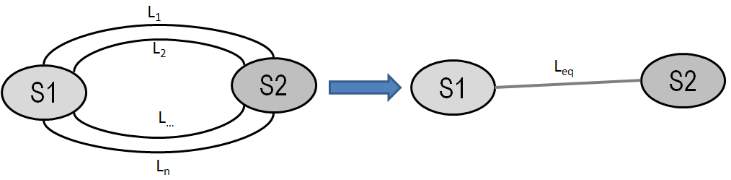
\includegraphics[width=.50\linewidth,height=.15\textheight,keepaspectratio]{images/image151.png}
\[
\left\{\mathcal V_{2/1}^{L_{\mathrm{eq}}}\right\}
=
\left\{\mathcal V_{2/1}^{L_1}\right\}
=
\left\{\mathcal V_{2/1}^{L_2}\right\}
=\cdots=
\left\{\mathcal V_{2/1}^{L_n}\right\}.
\]
\end{center}

Le torseur de la liaison équivalente doit être compatible avec tous les
torseurs des liaisons en parallèle.

\subsection{Liaisons en série avec les torseurs}

Les liaisons sont en série lorsqu'elles sont disposées à la suite les unes
des autres par l'intermédiaire de \(n-1\) CEC.

\begin{center}
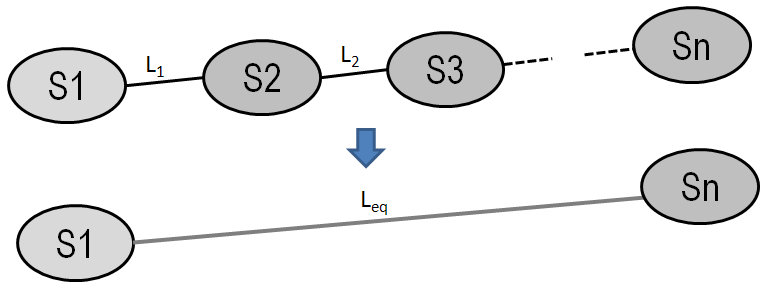
\includegraphics[width=.50\linewidth,height=.15\textheight,keepaspectratio]{images/image153.png}
\[
\left\{\mathcal V_{n/1}^{L_{\mathrm{eq}}}\right\}
=
\left\{\mathcal V_{n/n-1}^{L_n}\right\}
+\cdots+
\left\{\mathcal V_{3/2}^{L_2}\right\}
+\left\{\mathcal V_{2/1}^{L_1}\right\}.
\]
\end{center}

La liaison équivalente présente les degrés de liberté qui n'ont été supprimés
par aucune des liaisons de la chaîne.

% -----------------------------------------------------------------------------
\section{Sources}\TLSectionLabel{7}

Ce cours reprend et organise des ressources provenant notamment de Jacques
Le Goff, Corentin Kerzreho, Stéphane Génouel, de documents industriels
publics et d'activités pédagogiques de collègues de l'UPSTI.



% Les exercices possèdent leur propre bandeau historique. On expédie d'abord
% la dernière page du cours, puis on retire son bandeau avant les exercices.
\clearpage
\ClearShipoutPictureFG
% ============================================================================
% EXERCICES DU CHAPITRE
% Le fichier historique contient l'intégralité de la conversion Word.
% On n'exécute que la partie à partir de \section{Exercices du chapitre}.
% ============================================================================

\begingroup
\small
\sloppy
\setlength{\tabcolsep}{3pt}
\setlength{\LTleft}{0pt}
\setlength{\LTright}{0pt}
\setlength{\extrarowheight}{1pt}

% -----------------------------------------------------------------------------
% Images de l'ancienne conversion Word
% -----------------------------------------------------------------------------
\NewCommandCopy\TLLegacyIncludeGraphics\includegraphics

\NewDocumentCommand{\TLLegacyRawGraphic}{s O{} m}{%
  \ifstrempty{#2}{%
    \IfBooleanTF{#1}
      {\TLLegacyIncludeGraphics*[width=\linewidth,height=.82\textheight,keepaspectratio]{#3}}
      {\TLLegacyIncludeGraphics[width=\linewidth,height=.82\textheight,keepaspectratio]{#3}}%
  }{%
    \IfBooleanTF{#1}
      {\TLLegacyIncludeGraphics*[#2]{#3}}
      {\TLLegacyIncludeGraphics[#2]{#3}}%
  }%
}

\newcommand{\TLLegacyMissingGraphic}[1]{%
  \begin{tikzpicture}[baseline=(current bounding box.center)]
    \node[
      draw=TLCoverBlue!55,
      rounded corners=1mm,
      fill=TLCoverBlue!4,
      text=TLCoverBlue!80!black,
      align=center,
      font=\sffamily\scriptsize,
      inner sep=2mm,
      text width=24mm
    ] {Illustration vectorielle\\non convertie\\\ttfamily #1};
  \end{tikzpicture}%
}

\newcommand{\TLLegacyPlaceGraphic}[1]{%
  \ifinner
    \adjustbox{max width=.92\linewidth,max totalheight=.72\textheight}{#1}%
    \hspace{0pt}\allowbreak
  \else
    \par\noindent
    \makebox[\linewidth][c]{%
      \adjustbox{max width=.96\linewidth,max totalheight=.82\textheight}{#1}%
    }%
    \par\noindent
  \fi
}

\makeatletter
\RenewDocumentCommand{\includegraphics}{s O{} m}{%
  \begingroup
  \filename@parse{#3}%
  \edef\TLLegacyGraphicExtension{\filename@ext}%
  \edef\TLLegacyGraphicStem{\filename@area\filename@base}%

  \ifboolexpr{
    test {\ifstrequal{\TLLegacyGraphicExtension}{emf}}
    or test {\ifstrequal{\TLLegacyGraphicExtension}{EMF}}
    or test {\ifstrequal{\TLLegacyGraphicExtension}{wmf}}
    or test {\ifstrequal{\TLLegacyGraphicExtension}{WMF}}
  }{%
    \IfFileExists{\TLLegacyGraphicStem.png}{%
      \IfBooleanTF{#1}
        {\TLLegacyPlaceGraphic{\TLLegacyRawGraphic*[#2]{\TLLegacyGraphicStem.png}}}
        {\TLLegacyPlaceGraphic{\TLLegacyRawGraphic[#2]{\TLLegacyGraphicStem.png}}}%
    }{%
      \IfFileExists{\TLLegacyGraphicStem.pdf}{%
        \IfBooleanTF{#1}
          {\TLLegacyPlaceGraphic{\TLLegacyRawGraphic*[#2]{\TLLegacyGraphicStem.pdf}}}
          {\TLLegacyPlaceGraphic{\TLLegacyRawGraphic[#2]{\TLLegacyGraphicStem.pdf}}}%
      }{%
        \IfFileExists{\TLLegacyGraphicStem.jpeg}{%
          \IfBooleanTF{#1}
            {\TLLegacyPlaceGraphic{\TLLegacyRawGraphic*[#2]{\TLLegacyGraphicStem.jpeg}}}
            {\TLLegacyPlaceGraphic{\TLLegacyRawGraphic[#2]{\TLLegacyGraphicStem.jpeg}}}%
        }{%
          \IfFileExists{\TLLegacyGraphicStem.jpg}{%
            \IfBooleanTF{#1}
              {\TLLegacyPlaceGraphic{\TLLegacyRawGraphic*[#2]{\TLLegacyGraphicStem.jpg}}}
              {\TLLegacyPlaceGraphic{\TLLegacyRawGraphic[#2]{\TLLegacyGraphicStem.jpg}}}%
          }{%
            \TLLegacyPlaceGraphic{\TLLegacyMissingGraphic{\filename@base}}%
          }%
        }%
      }%
    }%
  }{%
    \IfBooleanTF{#1}
      {\TLLegacyPlaceGraphic{\TLLegacyRawGraphic*[#2]{#3}}}
      {\TLLegacyPlaceGraphic{\TLLegacyRawGraphic[#2]{#3}}}%
  }%
  \endgroup
}

\CatchFileDef{\TLLegacyModelisationFile}
  {02_ModelisationMecanismes_cours.tex}
  {}

% Les trois EMF ci-dessous se trouvent réellement dans la partie exercices.
% On les neutralise avant exécution du fichier capturé : pdfLaTeX ne voit donc
% jamais leur extension. image174 est une petite puce décorative ; les deux
% autres emplacements restent matérialisés par un repère discret.
\patchcmd{\TLLegacyModelisationFile}
  {
\includegraphics[width=\linewidth]{images/image174.emf}}
  {}
  {}{}
\patchcmd{\TLLegacyModelisationFile}
  {\protect
\includegraphics{images/image194.emf}}
  {\TLLegacyMissingGraphic{image194}}
  {}{}
\patchcmd{\TLLegacyModelisationFile}
  {
\includegraphics[width=\linewidth]{images/image220.emf}}
  {\TLLegacyMissingGraphic{image220}}
  {}{}

% Les images 158 et 159 étaient chacune demandées à \linewidth sur la même
% ligne. On les compose explicitement à 46 % de la largeur.
\patchcmd{\TLLegacyModelisationFile}
  {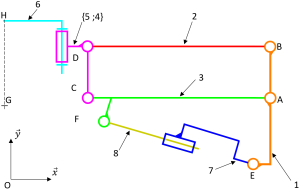
\includegraphics[width=\linewidth]{images/image158.png}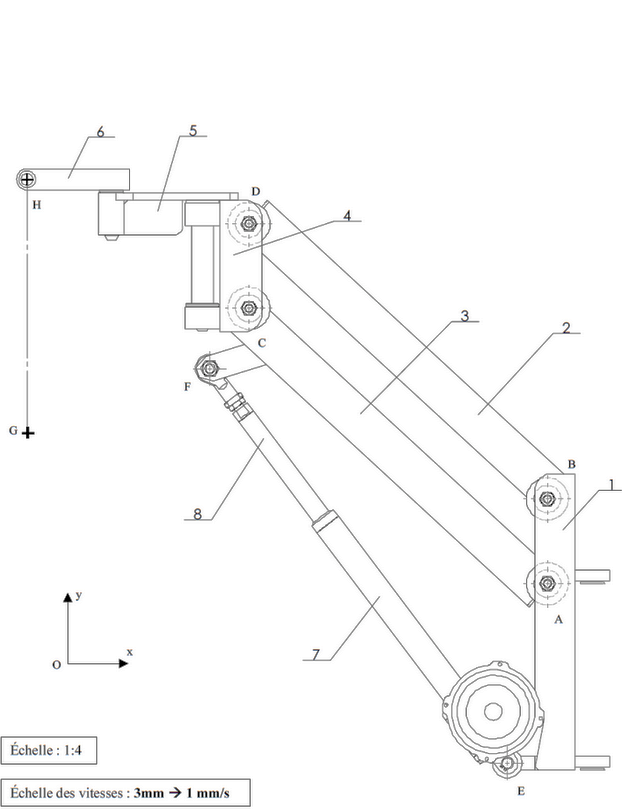
\includegraphics[width=\linewidth]{images/image159.png}}
  {\begin{center}%
   \TLLegacyIncludeGraphics[width=.46\linewidth]{images/image158.png}\hfill
   \TLLegacyIncludeGraphics[width=.46\linewidth]{images/image159.png}%
   \end{center}}
  {}{}

% Parcours récursif des commandes section du fichier capturé.
\long\def\TLExtractModelisationExercises#1\section#2#3\TLModelisationStop{%
  \ifstrequal{#2}{Exercices du chapitre}{%
    \section{#2}#3%
  }{%
    \expandafter\TLExtractModelisationExercises#3\TLModelisationStop
  }%
}

\expandafter\TLExtractModelisationExercises
  \TLLegacyModelisationFile
  \TLModelisationStop
\makeatother
\endgroup

